\documentclass[12pt,a4paper]{article}
\usepackage{myStyle}

\usepackage{fancyhdr}
\pagestyle{fancy}
\renewcommand{\headrulewidth}{0pt}
\fancyhf{}
\chead{
\includegraphics[width=1cm]{./img/logo.png}}
\setlength\headheight{28pt} 
\lfoot{Protocol version 1, day month year}
\rfoot{\thepage}

% Graphicspath used to avoid trouble with paths. 
% Change to approriate path when starting project.
\graphicspath{{/home/martin/Dropbox/sketchbook/python/project/project_template/protocol/img/}}

\begin{document}

\pagenumbering{arabic}
\setcounter{page}{1}

\section*{Title}
The best study in the world

\section*{Investigators}
Joanna Diong\textsuperscript{1} \\
Agatha Christie\textsuperscript{2} 

\textsuperscript{1}University of Sydney \\
\textsuperscript{2}University of Exeter

\section*{Introduction}
This study needs to be done \citep{Pascoe2014}

\subsection*{Aims}
The whole point of it is this:

\section*{Methods}

\textit{Participants} Data will be collected ... Participants will be recruited if they:
\begin{enumerate}
	\item have what it takes
	\item say yes
\end{enumerate}

\textit{Sample size} A sample size of N per group provides 80\% power to detect a between-groups effect of 5\% with standard deviation 7\% and alpha = 0.05.

\textit{Procedures} During testing, subjects were positioned ...

\begin{figure}[!htbp]
\centering
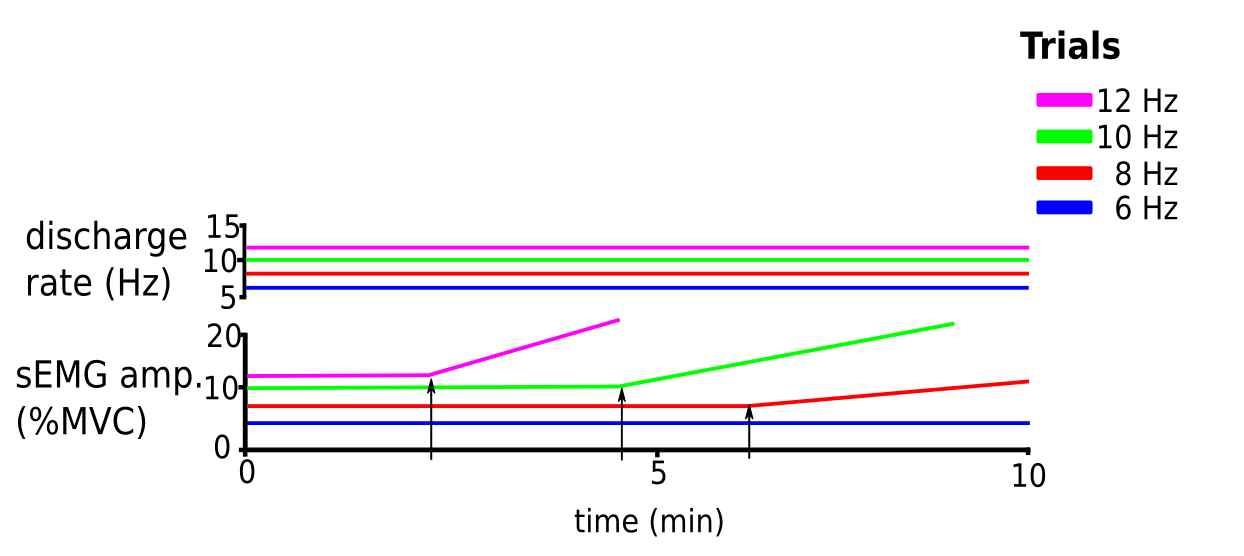
\includegraphics[scale=0.75]{./img/fake_data.png}
\captionsetup{justification=centering}
\caption{Fake data}
\end{figure}

\textit{Analysis} Between-groups effects were calculated with linear regression adjusting for age and segment length ...

% References:
\newpage
\bibliographystyle{./ref/jneurophysiol}
\bibliography{./ref/ref_list}
 
\end{document}
